\documentclass[a4paper]{article}
\usepackage{zadaci}
\usepackage{wrapfig}
\usepackage{url}
\usepackage{tikz}
\usepackage{amsmath}
\usepackage[normalem]{ulem}
\usetikzlibrary{angles,quotes}
\contestname{Croatian Open Competition in Informatics\\Round 5, February 8\textsuperscript{th} 2020}
\markright{\textbf{\textsf{Editorial}}}

\usepackage{hyperref}
\hypersetup{
colorlinks=true,
linkcolor=blue,
filecolor=magenta,
urlcolor=cyan,
}

\begin{document}

\section*{Editorial}

Tasks, test data and solutions were prepared by: Nikola Dmitrović, Karlo
Franić, Gabrijel Jambrošić, Marin Kišić, Daniel Paleka, Ivan Paljak and Paula
Vidas. Implementation examples are given in attached source code files.

\subsection*{Task: Emacs}
\textsf{Suggested by: Paula Vidas}\\
\textsf{Necessary skills: implementation}

The number of rectangles in the image is equal to the number of upper-left
corners of rectangles in the image. Cell $(i, j)$ is an upper-left corner of
some rectangle if that cell contains the character \texttt{'*'} while cells $(i
- 1, j)$ and $(i, j - 1)$ (if they exist) contain the character \texttt{'.'}.

Alternatively, we can use BFS to find the number of connected components in four
general directions which contain the character \texttt{'*'}.

\subsection*{Task: Političari}
\textsf{Suggested by: Ivan Paljak}\\
\textsf{Necessary skills: cycle detection}

It was possible to score $50\%$ ($35$) of total points on this task
simply by implementing what was described in the task statement. In other
words, you should have correctly implemented the rules by which politicians
blame each other until we reach the $K$-th show. The time complexity of this
solution is $\mathcal{O}(K)$, and the implementation details can be seen
in \texttt{politicari\_brute.cpp}.

To score all points on this task it was necessary to observe that the blaming
process is cyclical. Since the next guest on a talk show solely depends on the
previous guest and the person who blamed the previous guest, we can conclude
that there are at most $\mathcal{O}(N^2)$ different shows (states). We consider
two shows to be the same if they have the same guest that was blamed by the
same politician in the previous show. Otherwise, the shows are considered
different.

Since the total number of different shows is considerably less than the maximum
episode in which we are interested in, we can simulate the process until we
reach the show we have seen before (already visited state). At that moment,
assuming that we keep track of some key items that have happened, we can use
the power of math to calculate who will be the guest of the $K$-th show.

Let's assume we have realized that the $i$-th show will be the same as a
(some prior) $j$-th show. In that case, we have just entered a cycle of
length $(i-j)$ and can conclude that the guest which appeared in $(j + ((K -
j) \% (i - j)))$-th show will also appear in the $K$-th show. Here, we
use the $\%$ character to denote the modulo operator.

Time complexity of described solution is $\mathcal{O}(N^2)$.

\subsection*{Task: Holding}
\textsf{Suggested by: Fabijan Bošnjak and Marin Kišić}\\
\textsf{Necessary skills: dynamic programming, memory optimizations}

The solution of the first subtask is based on dynamic programming where the
state is a bitmask. We leave the rest of the details as a practice to the reader.

In the second subtask it is known that $R = N$, which means that we can swap
numbers on positions $L$, $L+1$, \dots, $R$ only with numbers on positions from
$1$ to $L-1$ (the rest of the solution assumes that the word \textit{interval}
refers to the agreed interval $L$, $L+1$, \dots, $R$). The first important observation
is that we will never change the position of a certain number more than once. The
second important observation, and much less obvious than the first, is that we
only care about which elements were chosen to be swapped within the interval and which were
chosen to be swapped outside the interval. Regardless of the way in which we have
swapped these numbers, their total cost will remain invariant. For example, if we
decided to swap positions $i$ and $j$ from within the interval with positions $k$
and $l$ that are outside the interval, it doesn't matter whether we have changed
$i$ with $k$ and $j$ with $l$ or $i$ with $l$ and $j$ with $k$. We leave the
formal proof of this claim as an exercise to the reader.

\begin{figure}[!htbp]
\centering
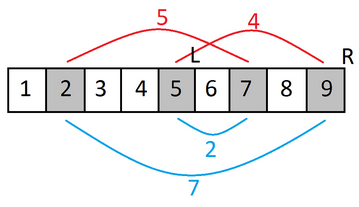
\includegraphics[width=0.4\textwidth]{editorial_holding.png}
\end{figure}

Now it is obvious that the only important thing left is to decide which elements
should be chosen from inside and which elements should be chosen from outside
of the interval and that the number of chosen elements from inside equals the
number of chosen elements outside of interval. We can achieve that using $dp$
whose arguments are the current position outside the interval, current position
inside the interval and the total amount of money we have spent thus far. The
$dp$ function returns the maximum decrease in sum of elements in our interval.
The initial state of $dp$ is $dp(1, L, 0)$ and the state where we will find our
solution is $dp(L - 1, R, K)$.

\begin{multline}
  dp(poz_{out}, poz_{in}, spent) = \max \biggl\{ dp(poz_{out} - 1, poz_{in}, spent),
  dp(poz_{out}, poz_{in} - 1, spent),\\
  dp(poz_{out} - 1, poz_{in} - 1, spent - (poz_{in} - poz_{out})) + A[poz_{in}] - A[poz_{out}] \biggr\}
\end{multline}

The first $dp$ transition tells us not to take an element on position $poz_{out}$,
the second transition tells us not to take an element on position $poz_{in}$, while
the third transition tells us to take both elements and swap them, thus spending
$poz_{in} - poz_{out}$ kunas.

The complexity of this algorithm is $\mathcal{O}(N^2 \cdot K)$.

This algorithm is therefore fast enough for the whole solution, but doesn't
include the swaps from the right side of the interval because $R=N$. Suppose
that the optimal solution takes $X$ elements left of the interval, $Y$ elements
right of the interval and $X+Y$ elements from inside the interval. It is obvious
that, if we sort positions of elements we took from within the interval, first
$X$ elements will be swapped with the $X$ chosen elements on the left side and
next $Y$ elements will be swapped with the $Y$ chosen elements on the right side.
This leads us to a conclusion that there is a line between positions within the
interval which determines that all elements from the interval left of that line
will be swapped with chosen elements left of the interval, and vice versa for
the right side. Since we don't know where that line might lie and since we
don't actually care how many swaps are made on each side of an interval, we
can to place that line on each position within the interval. We can do that
with the following lines of code:

\vspace{-2ex}
\begin{verbatim}
for i in range (L - 1, R+1):
  for j in range (0, K + 1):
    sol = max(sol, dpL(L - 1, i, j) + dpR(R + 1, i + 1, K - j))
\end{verbatim}

What are $dpL$ and $dpR$? $dpL$ is the same $dp$ from the last subtask and
$dpR$ is completely identical to it but is being done from the other side. The
complexity of each $dp$ is $\mathcal{O}(N^2 \cdot K)$ and the complexity of
merging their solutions is $\mathcal{O}(N \cdot K)$. Therefore, the total
complexity of the algorithm is $\mathcal{O}(N^2 \cdot K)$.

Why can't you score all the points with that solution then? Because tridimensional
array of the form \texttt{int dp[N][N][K]} takes up too much memory for $N = 100$, but it
fits for $N=50$. Therefore, we still need to optimize our memory consumption.
There are multiple ways to achieve that, but perhaps the easiest is to note that,
in the worst case for any $N$, $L$ and $R$, the maximum amount of money Ivica
needs to perform all swaps is going to be bounded by $\frac{N^2}{4}$. Luckily,
arrays of the form \texttt{int dp[N][N][N*N/4]} fit into the given memory limit
of \texttt{256 MiB}. There is another optimization which swaps the dimension $N$
with a smaller constant, you can check the implementation of that optimization
in the attached source code.

\subsection*{Task: Klasika}
\textsf{Suggested by: Ivan Paljak}\\
\textsf{Necessary skills: dfs tree traversal, trie}

The first two subtasks were solvable by more or less efficient attempts
to simulate the process described in the task statement. We will leave
further analysis of those solutions as exercises to the reader.

In the third subtask you were supposed to answer each \texttt{Query} with
the longest path in a tree which starts on given node $a$. Note that the
definition of path length is a bit peculiar, i.e. instead of summing up
the edge weights, we are asked to \texttt{xor} them. Let's denote the distance
between nodes $x$ and $y$ with $d(x,y)$. Note that $d(x, y) = d(1, x)$ \texttt{xor}
$d(1, y)$ holds for each pair of nodes. We can use this property and keep around
the distance from the root to each of the nodes while executing the queries.
Finding the greatest distance from a given node $a$ now boils down to finding
another value $d(1, b)$ from the set of remembered values which when \texttt{xor}-ed
with $d(1, a)$ gives a maximal value. This is a well-known problem which can be
easily solved using the \textit{trie} data structure. If you are not familiar with
the problem, we suggest you try to find the solution by yourself. If you don't
succeed, check out
 \href{https://www.hackerearth.com/practice/notes/lalitkundu95/tutorial-on-trie-and-example-problems/}{this link}.

The solution which scores all points is conceptually very similar to the
one described above. The only problem we are having is that, when we traverse
the trie, we don't know whether that part of the trie holds any value that
is related to a node that is in a subtree of node $b$. Imagine that we know
the values \texttt{discovery} and \texttt{finish} for each node which represent
the moments when a dfs traversal function enters and leaves that particular node.
Suppose that in each trie node we store a set of discovery times of all tree
nodes whose distances from the root live in that subtree of our trie. Then we
could simply make sure never to enter a trie node that doesn't hold a value
related to subtree of node $b$ while processing the \texttt{Query}. More
precisely, we can traverse a node in a trie if its set of discovery times
contains a value that is greater or equal to \texttt{discovery[b]} and
less or equal to \texttt{finish[b]}.

Turns out this is relatively easy to achieve. First we will apply all
\texttt{Add} queries (offline) and use a single dfs traversal to find
\texttt{discovery} and \texttt{finish} values for each node. Then we will
traverse through all queries once more and perform the algorithm described
above. When adding a new element to the trie, we will simply append the
corresponding \texttt{discovery} value to each of the visited trie nodes.
Finally, when answering a query we will make sure we don't visit trie
nodes that don't contain values related to the subtree of node $b$.

\subsection*{Task: Nivelle}
\textsf{Suggested by: Daniel Paleka}\\
\textsf{Necessary skills: sliding window technique, two pointers}

We can implement a solution of time complexity $\mathcal{O}(N^2)$ which
for every substring calculates the number of different letters in it. If
we use the so-called sliding window technique, we need to keep track
how many times each letter appears and note each time when a new letter
starts or stops appearing. For implementation details, check the attached
(slower) source code.

Note that the numerator of the expression we want to minimize, i.e. the
number of different characters in a substring, can either be $1$, $2$, \dots,
$26$. Therefore, it is enough to fix its value in every possible way and
determine the largest possible substring which has exactly that many different
characters. Now we have $26$ values to compare and pick the smallest one.

A simple implementation calculates for each starting character the longest
substring which contains exactly $K$ different characters. If we calculate
for each character and each position the first next appearance of that
character, for each starting character we can quickly check $\le 26$ strings
which go to \textit{the next new character}.

\end{document}
%%% Local Variables:
%%% mode: latex
%%% mode: flyspell
%%% ispell-local-dictionary: "croatian"
%%% End:
